\documentclass{article}
\usepackage[dvipsnames]{xcolor}
\usepackage[utf8]{inputenc}
\usepackage{appendix}
\usepackage[T1]{fontenc}
\usepackage[italian]{babel}
\usepackage{siunitx} % Provides the \SI{}{} and \si{} command for typesetting SI units
\usepackage{graphicx} % Required for the inclusion of images
\usepackage{natbib} % Required to change bibliography style to APA
\usepackage{amsmath} % Required for some math elements
\usepackage{caption}
\usepackage{float}
\usepackage{import}
\setlength\parindent{0pt} % Removes all indentation from paragraphs
\usepackage{minted}

\title{\vspace{-2cm}Progetto di Tecnologie Informatiche per il Web} % Title
\author{Negri Riccardo} % Author name
\date{\today}

\begin{document}

\maketitle

\begin{figure}[H]
\centering

\includegraphics[width=0.365\textwidth]{assets/logo.jpg}
\end{figure}

\begin{center}
\begin{tabular}{l l l l}
Docente: & Fraternali Piero& & \\ 
Studente: & Negri Riccardo & 10729927 & 936820 
\end{tabular}
\end{center}

\tableofcontents
\pagebreak

\section{Specifiche}

\subsection{Versione pure HTML}
Un’applicazione web consente la gestione di trasferimenti di denaro online da un conto a un
altro. L’applicazione supporta registrazione e login mediante una pagina pubblica con
opportune form. La registrazione controlla la validità sintattica dell’indirizzo di email e
l’uguaglianza tra i campi “password” e “ripeti password”. La registrazione controlla l’unicità
dello username. Un utente ha un nome, un cognome, uno username e uno o più conti correnti.
Un conto ha un codice, un saldo, e i trasferimenti fatti (in uscita) e ricevuti (in ingresso) dal
conto. Un trasferimento ha una data, un importo, un conto di origine e un conto di destinazione.
Quando l’utente accede all’applicazione appare una pagina LOGIN per la verifica delle
credenziali. In seguito all’autenticazione dell’utente appare l’HOME page che mostra l’elenco
dei suoi conti. Quando l’utente seleziona un conto, appare una pagina STATO DEL CONTO
che mostra i dettagli del conto e la lista dei movimenti in entrata e in uscita, ordinati per data
discendente. La pagina contiene anche una form per ordinare un trasferimento. La form
contiene i campi: codice utente destinatario, codice conto destinatario, causale e importo.
All’invio della form con il bottone INVIA, l’applicazione controlla che il conto di destinazione
appartenga all’utente specificato e che il conto origine abbia un saldo superiore o uguale
all’importo del trasferimento. In caso di mancanza di anche solo una condizione, l’applicazione
mostra una pagina con un avviso di fallimento che spiega il motivo del mancato trasferimento.
Nel caso in cui entrambe le condizioni siano soddisfatte, l’applicazione deduce l’importo dal
conto di origine, aggiunge l’importo al conto di destinazione e mostra una pagina CONFERMA
TRASFERIMENTO che presenta i dati dell’importo trasferito e i dati del conto di origine e di
destinazione con i rispettivi saldi precedenti al trasferimento e aggiornati dopo il trasferimento.
L’applicazione deve garantire l’atomicità del trasferimento: ogni volta che il conto di
destinazione viene addebitato, il conto di origine deve essere accreditato. Ogni pagina
contiene un collegamento per tornare alla pagina precedente. L’applicazione consente il
logout dell’utente.

\pagebreak
\subsection{Versione RIA}
Si realizzi un’applicazione client server web che modifica le specifiche precedenti come segue:
\begin{itemize}
\item La registrazione controlla la validità sintattica dell’indirizzo di email e l’uguaglianza tra
i campi “password” e “ripeti password”, anche a lato client.
\item Dopo il login, l’intera applicazione è realizzata con un’unica pagina.
\item 	Ogni interazione dell’utente è gestita senza ricaricare completamente la pagina, ma
produce l’invocazione asincrona del server e l’eventuale modifica del contenuto da
aggiornare a seguito dell’evento.
\item I controlli di validità dei dati di input (ad esempio importo non nullo e maggiore di zero)
devono essere realizzati anche a lato client.
\item L’avviso di fallimento è realizzato mediante un messaggio nella pagina che ospita
l’applicazione.
\item L’applicazione chiede all’utente se vuole inserire nella propria rubrica i dati del
destinatario di un trasferimento andato a buon fine non ancora presente. Se l’utente
conferma, i dati sono memorizzati nella base di dati e usati per semplificare
l’inserimento. Quando l’utente crea un trasferimento, l’applicazione propone mediante
una funzione di auto-completamento i destinatari in rubrica il cui codice corrisponde
alle lettere inserite nel campo codice utente destinatario.
\end{itemize}

\pagebreak
\section{Database design}

\subsection{Analisi testo delle specifiche}
Legenda: \textcolor{red}{entità}, \textcolor{ForestGreen}{attributi}, \textcolor{blue}{relazioni}.
\\
\\
Un’applicazione web consente la gestione di trasferimenti di denaro online da un conto a un
altro. L’applicazione supporta registrazione e login mediante una pagina pubblica con
opportune form. La registrazione controlla la validità sintattica dell’\textcolor{ForestGreen}{indirizzo di email} e
l’uguaglianza tra i campi “\textcolor{ForestGreen}{password}” e “ripeti password”. La registrazione controlla l’unicità
dello username. Un \textcolor{red}{utente} ha un \textcolor{ForestGreen}{nome}, un \textcolor{ForestGreen}{cognome}, uno \textcolor{ForestGreen}{username} e \textcolor{blue}{uno o più conti correnti}.
Un \textcolor{red}{conto}  ha un \textcolor{ForestGreen}{codice}, un \textcolor{ForestGreen}{saldo}, e i \textcolor{blue}{trasferimenti fatti (in uscita) e ricevuti (in ingresso)} dal
conto. Un  \textcolor{red}{trasferimento} ha una \textcolor{ForestGreen}{data}, un \textcolor{ForestGreen}{importo}, un \textcolor{blue}{conto di origine e un conto di destinazione}.
Quando l’utente accede all’applicazione appare una pagina LOGIN per la verifica delle
credenziali. In seguito all’autenticazione dell’utente appare l’HOME page che mostra l’elenco
dei suoi conti. Quando l’utente seleziona un conto, appare una pagina STATO DEL CONTO
che mostra i dettagli del conto e la lista dei movimenti in entrata e in uscita, ordinati per data
discendente. La pagina contiene anche una form per ordinare un trasferimento. La form
contiene i campi: codice utente destinatario, codice conto destinatario, \textcolor{ForestGreen}{causale} e importo.
All’invio della form con il bottone INVIA, l’applicazione controlla che il conto di destinazione
appartenga all’utente specificato e che il conto origine abbia un saldo superiore o uguale
all’importo del trasferimento. In caso di mancanza di anche solo una condizione, l’applicazione
mostra una pagina con un avviso di fallimento che spiega il motivo del mancato trasferimento.
Nel caso in cui entrambe le condizioni siano soddisfatte, l’applicazione deduce l’importo dal
conto di origine, aggiunge l’importo al conto di destinazione e mostra una pagina CONFERMA
TRASFERIMENTO che presenta i dati dell’importo trasferito e i dati del conto di origine e di
destinazione con i rispettivi saldi precedenti al trasferimento e aggiornati dopo il trasferimento.
L’applicazione deve garantire l’atomicità del trasferimento: ogni volta che il conto di
destinazione viene addebitato, il conto di origine deve essere accreditato. Ogni pagina
contiene un collegamento per tornare alla pagina precedente. L’applicazione consente il
logout dell’utente.

\subsection{Progetto concettuale - Diagramma E-R (Entità-Relazione)}
Da aggiornare - deve esistere sempre un conto associato ad un utente, anche quando si registra
\begin{figure}[H]
\centering
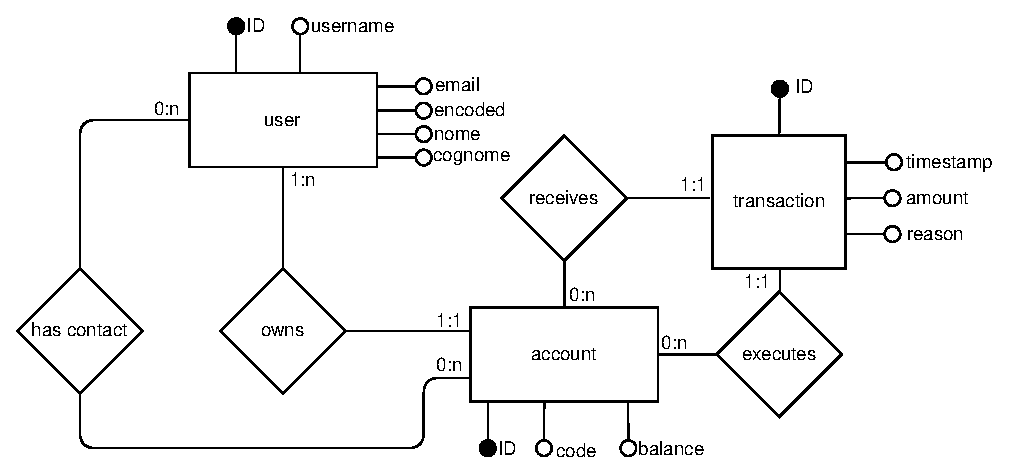
\includegraphics[width=1\textwidth]{assets/diagram.eps}
\end{figure}

\subsection{Progetto logico}
UTENTE(\underline{ID}, username, email, password, nome, cognome)
\\
CONTO(\underline{ID}, codice, saldo, utente)
\\
TRASFERIMENTO(\underline{ID}, data, importo, causale, origine, destinazione)

\subsection{Database schema}
Statement per creare il database:
\begin{minted}{mysql}
CREATE DATABASE tiw_db;
\end{minted}

Statements per creare le tabelle:
\begin{minted}{mysql}
CREATE TABLE `tiw_db`.`user` (
	`id` INT NOT NULL AUTO_INCREMENT,
	`username` VARCHAR(45) NOT NULL UNIQUE,
	`email` VARCHAR(45) NOT NULL UNIQUE,
	`password` VARCHAR(45) NOT NULL,
	`name` VARCHAR(45) NOT NULL,
	`surname` VARCHAR(45) NOT NULL,
	PRIMARY KEY (`id`)
);

\end{minted}
\pagebreak
\begin{minted}{mysql}
CREATE TABLE `tiw_db`.`account` (
	`id` INT NOT NULL AUTO_INCREMENT,
	`code` VARCHAR(12) NOT NULL UNIQUE,
	`balance` FLOAT NOT NULL DEFAULT 0,
	`user` INT NOT NULL,
	PRIMARY KEY (`id`),
	CONSTRAINT `user_account` FOREIGN KEY (`user`) 
		REFERENCES `tiw_db`.`user` (`id`) 
			ON DELETE NO ACTION ON UPDATE CASCADE
);
\end{minted}

\begin{minted}{mysql}
CREATE TABLE `tiw_db`.`transaction` (
	`id` INT NOT NULL AUTO_INCREMENT,
	`timestamp` DATETIME DEFAULT CURRENT_TIMESTAMP,
	`amount` INT NOT NULL,
	`reason` VARCHAR(255) NOT NULL,
	`origin` INT NOT NULL,
	`destination` INT NOT NULL,
	PRIMARY KEY (`id`),
	CONSTRAINT `transaction_origin` FOREIGN KEY (`origin`) 
		REFERENCES `tiw_db`.`account` (`id`)
			ON DELETE NO ACTION ON UPDATE CASCADE,
	CONSTRAINT `transaction_destination` FOREIGN KEY (`destination`) 
		REFERENCES `tiw_db`.`account` (`id`) 
			ON DELETE NO ACTION ON UPDATE CASCADE
);
\end{minted}

\subsection{Script Python per popolare il database}
Al fine di popolare automaticamente un nuovo database è stato creato uno script in Python chiamato "populate-tiw-db.py." 

\section{Versione pure HTML}

\subsection{Analisi requisiti delle specifiche}
Legenda: \textcolor{red}{pagine}, \textcolor{ForestGreen}{view components}, \textcolor{blue}{eventi}, \textcolor{brown}{azioni (modifca il db)}.
\\
\\
Un’applicazione web consente la gestione di trasferimenti di denaro online da un conto a un
altro. L’applicazione supporta  \textcolor{brown}{registrazione} e  \textcolor{blue}{login} mediante una pagina pubblica con
opportune  \textcolor{ForestGreen}{form}. La registrazione controlla la validità sintattica dell’indirizzo di email e
l’uguaglianza tra i campi “password” e “ripeti password”. La registrazione controlla l’unicità
dello username. Un utente ha un nome, un cognome, uno username e uno o più conti correnti.
Un conto ha un codice, un saldo, e i trasferimenti fatti (in uscita) e ricevuti (in ingresso) dal
conto. Un trasferimento ha una data, un importo, un conto di origine e un conto di destinazione.
Quando l’utente accede all’applicazione appare una  \textcolor{red}{pagina LOGIN} per la verifica delle
credenziali. In seguito all’autenticazione dell’utente appare \textcolor{red}{l’HOME page} che \textcolor{ForestGreen}{mostra l’elenco
dei suoi conti}. Quando l’utente  \textcolor{blue}{seleziona un conto}, appare una \textcolor{red}{pagina STATO DEL CONTO}
che mostra i \textcolor{ForestGreen}{dettagli del conto e la lista dei movimenti in entrata e in uscita}, ordinati per data
discendente. La pagina contiene anche una \textcolor{ForestGreen}{form} per ordinare un trasferimento. La form
contiene i campi: codice utente destinatario, codice conto destinatario, causale e importo.
All’invio della form con il bottone INVIA, l’applicazione controlla che il conto di destinazione
appartenga all’utente specificato e che il conto origine abbia un saldo superiore o uguale
all’importo del trasferimento. In caso di mancanza di anche solo una condizione, l’applicazione
mostra una \textcolor{red}{pagina con un avviso di fallimento} che spiega il motivo del mancato trasferimento.
Nel caso in cui entrambe le condizioni siano soddisfatte, l’applicazione deduce l’importo dal
conto di origine, aggiunge l’importo al conto di destinazione e mostra una \textcolor{red}{pagina CONFERMA
TRASFERIMENTO} che presenta i dati dell’importo trasferito e i dati del conto di origine e di
destinazione con i rispettivi saldi precedenti al trasferimento e aggiornati dopo il trasferimento.
L’applicazione deve garantire l’atomicità del trasferimento: ogni volta che il conto di
destinazione viene addebitato, il conto di origine deve essere accreditato. Ogni pagina
contiene un collegamento per tornare alla pagina precedente. L’applicazione consente il
logout dell’utente.

\subsection{Completamento specifiche}

\section{Versione RIA}


\end{document}